% Bug closure time in open-source games (coursework report).
% Build:  cd report_source && tectonic main.tex
\documentclass[10pt,a4paper]{article}
\usepackage[margin=2.4cm]{geometry}
\usepackage{graphicx}
\usepackage{booktabs}
\usepackage{tabularx}
\usepackage{array}
\usepackage{amsmath}
\usepackage{amssymb}
\usepackage{xcolor}
\usepackage{caption}
\usepackage{cite}
\usepackage[hidelinks]{hyperref}
\usepackage{url}
\captionsetup{font=small, labelfont=bf}
\setlength{\parskip}{0.35em}
\setlength{\parindent}{0em}
\hyphenpenalty=1000
\emergencystretch=2em

% Float placement flexibility
\renewcommand{\topfraction}{0.90}
\renewcommand{\bottomfraction}{0.85}
\renewcommand{\textfraction}{0.10}
\renewcommand{\floatpagefraction}{0.80}
\setlength{\textfloatsep}{10pt plus 2pt minus 2pt}
\setlength{\intextsep}{8pt plus 2pt minus 2pt}
\setlength{\floatsep}{8pt plus 2pt minus 2pt}

% GENERATED by src/build_report.py -- do not edit by hand.
\newcommand{\valnA}{14,280}
\newcommand{\valnB}{662}
\newcommand{\valnC}{48,746}
\newcommand{\valmedA}{8.0}
\newcommand{\valmedB}{35.3}
\newcommand{\valmeanA}{110.6}
\newcommand{\valmeanB}{219.4}
\newcommand{\valqOneA}{1.51}
\newcommand{\valqThreeA}{54.4}
\newcommand{\valqOneB}{5.92}
\newcommand{\valqThreeB}{200.6}
\newcommand{\valpNinetyA}{280}
\newcommand{\valpNinetyB}{625}
\newcommand{\valmedDiff}{27.3}
\newcommand{\valUstat}{6\,069\,998}
\newcommand{\valpPrim}{3.31\times 10^{-35}}
\newcommand{\valpPrimOne}{1.66\times 10^{-35}}
\newcommand{\valcliffsD}{0.284}
\newcommand{\valcliffsMag}{small}
\newcommand{\valhlShift}{9.8}
\newcommand{\valciIssue}{[18.3, 35.2] days}
\newcommand{\valciCluster}{[13.9, 51.4] days}
\newcommand{\valnProjAB}{361}
\newcommand{\valnProjBoth}{117}
\newcommand{\valnBhigher}{88}
\newcommand{\valnBlower}{29}
\newcommand{\valsignP}{4.28\times 10^{-8}}
\newcommand{\valmedProjDiff}{24.4}
\newcommand{\valfeCoef}{0.905}
\newcommand{\valfeCI}{[0.671, 1.140]}
\newcommand{\valfeP}{3.83\times 10^{-14}}
\newcommand{\valfePct}{147}
\newcommand{\valfeN}{14,942}
\newcommand{\valfeProj}{361}
\newcommand{\valrho}{0.101}
\newcommand{\valrhoP}{1.72\times 10^{-35}}
\newcommand{\valkrustH}{158.7}
\newcommand{\valkrustP}{2.76\times 10^{-33}}
\newcommand{\valtMedLast}{95.3}
\newcommand{\valtNinety}{57.6}
\newcommand{\valtSeventyFive}{70.8}
\newcommand{\valtMedFirst}{27.7}
\newcommand{\valaFracMed}{83.5}
\newcommand{\valdetNA}{4,271}
\newcommand{\valdetNB}{108}
\newcommand{\valdetMedA}{3.3}
\newcommand{\valdetMedB}{12.0}
\newcommand{\valdetDiff}{8.6}
\newcommand{\valdetP}{6.44\times 10^{-12}}
\newcommand{\valdetD}{0.386}
\newcommand{\valkmAn}{12,672}
\newcommand{\valkmAopen}{276}
\newcommand{\valkmAmed}{8}
\newcommand{\valkmBn}{2,620}
\newcommand{\valkmBopen}{74}
\newcommand{\valkmBmed}{14}
\newcommand{\vallrChi}{43.8}
\newcommand{\vallrP}{3.62\times 10^{-11}}
\newcommand{\valSzero}{326,182}
\newcommand{\valSone}{73,035}
\newcommand{\valStwo}{63,688}
\newcommand{\valSfour}{63,688}
\newcommand{\vallabelsTotal}{4,273}
\newcommand{\vallabelsStrict}{33}
\newcommand{\vallabelsBroad}{75}
\newcommand{\vallabelsExcl}{4,165}
\newcommand{\valissBroad}{83,247}
\newcommand{\valsnapshot}{2025-10-12 22:28:19+09:00}
\newcommand{\valnProjCohort}{662}
\newcommand{\valnLinksCohort}{15,659}
\newcommand{\valmaxK}{8}
\newcommand{\valnExclStrict}{9,347}
\newcommand{\vallmCohort}{14,942}
\newcommand{\vallmAtRisk}{4,909}
\newcommand{\vallmClosed}{10,033}
\newcommand{\vallmNZero}{4,063}
\newcommand{\vallmNOne}{813}
\newcommand{\vallmNM}{33}
\newcommand{\vallmMedOne}{30.0}
\newcommand{\vallmMedM}{29.2}
\newcommand{\vallmDiff}{-0.8}
\newcommand{\vallmP}{0.832}
\newcommand{\vallmD}{-0.022}
\newcommand{\vallmCI}{[-22.5, 29.2] days}
\newcommand{\vallmMedZ}{136.4}
\newcommand{\vallmZP}{2.06\times 10^{-6}}
\newcommand{\vallmZD}{-0.479}
\newcommand{\vallmShareB}{90.4\%}
\newcommand{\vallmShareA}{84.5\%}
\newcommand{\vallmSignN}{22}
\newcommand{\vallmSignW}{13}
\newcommand{\vallmSignP}{0.523}
\newcommand{\valvN}{100}
\newcommand{\valvConf}{91}
\newcommand{\valvRej}{2}
\newcommand{\valvUnc}{7}
\newcommand{\valvPrec}{97.9\%}
\newcommand{\valvCI}{[92.5\%, 99.4\%]}
\newcommand{\valvPrecAll}{91.0\%}
\newcommand{\valvCIAll}{[83.8\%, 95.2\%]}


\title{\bfseries Linked Pull Requests and Bug Closure Time in Open-Source Games:\\ A Study of the OSSGameBench Dataset}
\author{\textbf{HASSANEEN Hassan} \\ Student ID: 661326003-0 \\ \textit{90355:Advanced Topics in Software Engineering}}
\date{}

\begin{document}
\maketitle
\begin{abstract}
\noindent
Bug reports in open-source games sometimes close after one pull request (PR) and sometimes after several. Do issues attracting multiple PRs really take longer to resolve, or do issues that stay open simply have more time to collect PR links? We analyse the OSSGameBench dataset (Version v2, Zenodo record 17553539, checksum verified): 326,182 issues across 970 open-source game repositories, focusing on 63,688 closed issues labelled as bugs. Among issues with at least one linked PR, 14,280 have exactly one (median 8.0 days to closure) and 662 have two or more (median 35.3 days). The association is statistically strong (median difference 27.3 days; Cliff's $\delta=0.284$; project-level 95\% CI 13.9--51.4 days) and survives seven robustness checks. Yet in multi-PR issues the last linked PR appears, at the median, at 95.3\% of the issue's observed lifetime. A fixed-landmark analysis fixing each issue's PR group at day~30 and comparing subsequent closure time finds essentially no difference (813 one-PR vs.\ 33 multi-PR issues; median difference $-0.8$ days, 95\% CI $-22.5$ to 29.2 days), and 90.4\% of multi-PR issues gained their second PR only after day~30. Much of the raw difference therefore reflects links accumulating while an issue stays open. We present practical maintainer recommendations and distinguish measured calendar duration from unmeasured developer effort.
\end{abstract}

\section{Introduction}\label{sec:intro}

Open-source game development represents a distinct engineering domain characterized by multidisciplinary assets (game logic, graphics, audio, shaders, and level data) and predominantly volunteer-driven development cycles~\cite{marsad2026ossgamebench}. When users and contributors encounter defects, issues are tracked in repository issue trackers, investigated, and addressed through pull requests (PRs)~\cite{gousios2014pull}. While many bug reports are resolved with a single PR, a subset accumulates multiple linked PRs over time. This multi-PR pattern can arise from various development workflows: modular decomposition of fixes across subsystems, abandoned initial attempts replaced by subsequent patches, or separate fixes for newly introduced regressions.

From a project management and triage perspective, maintainers naturally seek diagnostic signals: if issues attracting multiple PRs are systematically slower to close, observing a second PR could serve as an actionable trigger for maintainer re-triage. However, interpreting this relationship requires caution due to a fundamental methodological challenge: \emph{reverse causality via time-dependent link accumulation}. Because pull requests can only be linked to an issue while that issue remains open, longer-lived issues have substantially more calendar opportunity to accumulate PR references. An observed statistical association between multi-PR issues and prolonged closure times might simply reflect the passage of time rather than higher intrinsic defect difficulty.

Furthermore, empirical repository studies must rigorously separate observable trace data from unmeasured operational concepts:
\begin{enumerate}
  \item \textbf{Calendar Duration vs.\ Debugging Effort}: The elapsed calendar duration ($\texttt{closed\_at} - \texttt{created\_at}$) measures wall-clock time, which conflates active debugging with triage queues, contributor dormancy, review latency, and volunteer availability~\cite{mockus2002two}.
  \item \textbf{Issue Closure vs.\ Verified Fix}: Issue closure indicates an administrative state transition, which does not guarantee that the defect was successfully resolved or verified against regressions; issues are also closed due to obsolescence, duplicates, or lack of reproducibility~\cite{herzig2013not}.
  \item \textbf{Reported Bugs vs.\ Actual Defect Occurrence}: Issue trackers record reported and labelled defects, omitting unfiled bugs or informal patches.
\end{enumerate}

\textbf{Research Question (RQ).} We formulate our central inquiry:
\begin{quote}
\emph{Among closed, labelled bug issues in open-source games, is multi-PR resolution associated with longer issue closure times, and does this relationship reflect genuine workflow delay or time-dependent link accumulation?}
\end{quote}

\textbf{Contribution beyond prior work.} While the original OSSGameBench publication~\cite{marsad2026ossgamebench} introduced the dataset and described high-level repository distributions, it did not investigate bug resolution dynamics. This coursework study provides:
\begin{itemize}
  \item A rigorous cohort filtering pipeline isolating 63,688 closed strict bugs across 970 repositories.
  \item A rank-based comparison of single-PR vs.\ multi-PR closure times with project-clustered uncertainty estimation.
  \item An empirical PR-arrival timing analysis demonstrating that secondary PRs accumulate predominantly at the end of issue lifespans.
  \item A fixed-landmark survival analysis ($L=30$ days) that blocks the link-accumulation channel and evaluates the residual association.
  \item A 100-issue random sample audit evaluating bug-label precision.
  \item Actionable, grounded recommendations for open-source game maintainers, with explicit empirical boundaries.
\end{itemize}

\section{Dataset and Approach}\label{sec:data}

\subsection{The OSSGameBench Corpus}\label{sec:corpus}
We analyze the public \textbf{OSSGameBench} dataset~\cite{marsad2026ossgamebench}, a comprehensive empirical benchmark of contributor and development activities across 970 open-source video games and game development engines on GitHub. The dataset provides relational Apache Parquet tables capturing projects, issues, pull requests, comments, and commit associations, as well as an \texttt{issue\_pr} cross-reference table. In total, the corpus records \valSzero{} reported issues and 396,048 pull requests.

The dataset captures \emph{reported} issues and developer activity traces. Bugs fixed directly without corresponding issue tracker tickets, or issues opened as general questions or feature proposals, reflect maintainer workflow conventions. Consequently, the dataset enables empirical evaluation of the lifecycle of reported, labelled bug tickets.

\subsection{Dataset Version and Provenance Verification}\label{sec:provenance}
This study is conducted strictly on the **OSSGameBench dataset (Version v2)**, hosted under Zenodo record \texttt{17553539} (DOI: \texttt{10.5281/zenodo.17553539})~\cite{zenodo_ossgamebench_v2}. Before undertaking any data processing, the integrity of the downloaded corpus archive was verified against the cryptographic digest published in the Zenodo record:
\begin{equation}
\text{MD5}(\texttt{OSSGameBench.zip}) = \texttt{40fd064b56ec327b6284039b18b19ea1}
\end{equation}
The local archive verified as an exact cryptographic match. All Parquet tables were extracted and verified against their stored CRC-32 integrity records. Throughout the entire analysis pipeline, all raw dataset tables were accessed in read-only mode to guarantee complete reproducibility and eliminate any risk of data mutation.

\subsection{Data-Quality Inventory and Snapshot Boundaries}\label{sec:inventory}
Repository mining datasets inevitably encounter collection boundaries and metadata hygiene anomalies. Because GitHub snapshots do not include a formal cutoff header, we determine the effective snapshot boundary from the data: the latest observed event timestamp across all entity tables is \valsnapshot{} (UTC). Events occurring after this date cannot be observed, establishing the right-censoring boundary for issues still open at the snapshot date.

Timestamps follow the ISO-8601 standard with explicit timezone offsets; all dates were parsed using strict datetime conversions, routing unparseable records to an explicit exclusion ledger (\S\ref{sec:cohort}). Table~\ref{tab:inventory} presents verified entity counts and data-quality findings. Notably, the \texttt{issue\_pr} link table contains 8,961 exact duplicate link tuples and 3,694 link records referencing issue identifiers absent from the main issue entity table. Critically, GitHub's cross-referencing model records link relationships as static relational associations without event timestamps indicating \emph{when} a PR was linked to an issue. This data limitation directly motivates the design of our landmark analysis in \S\ref{sec:landmarkdesign}.

\begin{table}[t]
\centering
\caption{Selected inventory and data-quality findings for the OSSGameBench dataset (Version v2).\label{tab:inventory}}
\small \begin{tabular}{@{}ll@{}}
\toprule
Item & Value \\\midrule
Projects (project.parquet) & 970 \\
Issues & 326,182 (unique composite keys) \\
Issue comments & 853,302 \\
Pull requests & 396,048 \\
PR comments & 689,749 \\
issue\_pr link rows & 78,060 raw / 69,099 unique (8,961 exact duplicates) \\
pr\_commit rows & 1,565,625 \\
Commits in per-project detail files & 2,796,851 across 973 files \\
Distinct issue labels & 4,273 \\
Issues with no labels & 109,326 \\
Issue creation range & 2000-12-12 to 2025-10-12 \\
PR merge range & 2010-10-16 to 2025-10-12 \\
Links not resolving to issue.parquet & 3,694 \\
Links not resolving to pr.parquet & 137 \\
Malformed timestamps (all 5 datetime columns) & 0 \\
PRs with closed\_at $<$ created\_at & 1 \\
Comment tables expose created\_at? & no (see \S\ref{sec:threats}) \\
\bottomrule
\end{tabular}
\end{table}


\subsection{Methodological Pipeline}\label{sec:approach}
The investigation follows a fully scripted, reproducible execution workflow:
\begin{enumerate}
  \item \textbf{Data Ingestion \& Hygiene Audit}: Schema validation, timestamp consistency checks, and relational integrity verification.
  \item \textbf{Label Classification}: Categorization of all \vallabelsTotal{} distinct issue labels into deterministic taxonomy tiers.
  \item \textbf{Cohort Construction}: Multi-stage exclusion filtering of closed bug issues with unambiguous PR linkages.
  \item \textbf{Statistical Comparison}: Non-parametric hypothesis testing, robust effect sizes, and project-clustered bootstrap uncertainty intervals.
  \item \textbf{Survival and Landmark Modeling}: Decomposition of calendar delay vs.\ PR arrival timing, followed by a fixed-landmark analysis at $L=30$ days to isolate reverse causality.
  \item \textbf{Classification Validation}: A 100-issue sampled audit evaluating bug label precision.
  \item \textbf{Robustness Suite}: Seven sensitivity checks evaluating stability across classification, linkage, and project clustering definitions.
\end{enumerate}
All reproduction code and instructions are available in the replication package repository~\cite{replication_repo}.

\section{Measures and Analysis}\label{sec:method}

\subsection{Identifying Bugs: Label Taxonomy and Validation Audit}\label{sec:labels}
The OSSGameBench corpus does not contain ground-truth defect classifications; the primary signal is the set of label strings applied by repository maintainers. To identify reported bugs systematically, we extracted all \vallabelsTotal{} distinct label strings across the corpus and mapped them into three mutually exclusive tiers according to deterministic written rules:
\begin{enumerate}
  \item \textbf{Strict Tier} (\vallabelsStrict{} labels): Unambiguous bug assertions, including \texttt{bug}, \texttt{type: bug}, \texttt{defect}, and \texttt{kind/bug}. An issue is classified as a \emph{strict bug} if it carries at least one strict label (\valSone{} issues).
  \item \textbf{Broad Tier} (\vallabelsBroad{} labels): Symptom-oriented indicators (e.g., \texttt{crash}, \texttt{regression}, \texttt{freeze}). Retained exclusively for sensitivity testing (robustness check R1).
  \item \textbf{Excluded Tier} (\vallabelsExcl{} labels): Non-defect items (e.g., \texttt{enhancement}, \texttt{documentation}) and administrative tags like \texttt{duplicate} or \texttt{won't-fix}~\cite{herzig2013not}.
\end{enumerate}

\textbf{Label Validation Audit.} Because automated string rules can misclassify issues, we conducted a validation audit on a simple random sample of $n=\valvN$ issues drawn without replacement from the closed strict-bug cohort (fixed seed 20261120; all sampled issue IDs and reviewer notes are archived in the replication repository). We established a written operational defect definition prior to screening:
\begin{quote}
\emph{A bug report describes software behaviour that deviates from expected operation—incorrect computational results, crashes, engine freezes, visual or audio rendering glitches, or memory/resource leaks—as distinguished from requests for new features, configuration guidance, or build/CI maintenance.}
\end{quote}
Each sampled ticket (repository, title, and initial 1{,}200 characters of the body) was screened against this standard and marked \emph{confirmed}, \emph{rejected}, or \emph{uncertain}, accompanied by an explicit classification rationale.

\textbf{Transparency and reviewer identity.} In full accordance with reporting guidelines, this screening was conducted by a single investigator \textbf{assisted by an LLM}, rather than through two independent double-blind human coders. We therefore treat this as an automated, assisted audit rather than a human-only gold standard. This audit evaluates \emph{precision} (the proportion of tickets classified as strict bugs that represent true defects); it does not evaluate \emph{recall} (unlabelled defects omitted from the strict tier). Results are detailed in \S\ref{sec:validation}.

\subsection{Cohort Construction and Group Definitions}\label{sec:cohort}
From the full set of \valSzero{} reported issues, we apply sequential filtering: retaining strict bugs, requiring a recorded status of \texttt{CLOSED} with a valid ISO timestamp, and confirming non-negative duration ($\texttt{closed\_at} \ge \texttt{created\_at}$). Table~\ref{tab:stages} tracks the exclusion pipeline, culminating in \valSfour{} closed strict bugs across \valnProjCohort{} projects.

\begin{table}[t]
\centering
\caption{Cohort construction and filtering stages for closed strict bug issues.\label{tab:stages}}
\small \begin{tabular}{@{}lrl@{}}
\toprule
Stage & Issues & Retained \\\midrule
S0 & 326,182 & 100.0\% of S0\\
S1 & 73,035 & 22.4\% of S0\\
S2 & 63,688 & 19.5\% of S0\\
S3 & 63,688 & no change\\
S4 & 63,688 & 19.5\% of S0\\
\bottomrule
\end{tabular}
\end{table}


We define group membership based on the count of \emph{distinct, resolvable} linked pull requests referenced in the \texttt{issue\_pr} table:
\begin{itemize}
  \item \textbf{Group A (Single-PR)}: Exactly one resolvable linked PR ($n=\valnA$).
  \item \textbf{Group B (Multi-PR)}: Two or more resolvable linked PRs ($n=\valnB$, maximum observed $k=\valmaxK$).
  \item \textbf{Group C (No-PR)}: Zero resolvable linked PRs ($n=\valnC$). Group C issues represent the majority (76.5\%); they are analyzed descriptively but excluded from the primary comparative analysis, which addresses resolution dynamics among PR-linked issues.
\end{itemize}

\subsection{Outcome Operationalization: Duration vs.\ Debugging Effort}\label{sec:outcome}
The outcome metric is \emph{observed issue-to-closure duration}, measured in elapsed calendar days from \texttt{created\_at} to \texttt{closed\_at}. We emphasize that this metric reflects the elapsed calendar lifespan of a ticket. It is \textbf{not a direct measure of developer debugging effort}~\cite{mockus2002two}. Calendar duration conflates active technical investigation with queueing delays, waiting for user reproduction steps, maintainer holidays, code review latency, and release cycle scheduling. Furthermore, closure does not necessarily imply a verified bug fix~\cite{herzig2013not}. Throughout this paper, ``longer closure'' refers strictly to elapsed calendar duration.

\subsection{Comparative Statistical Framework}\label{sec:stats}
Because issue lifetimes exhibit extreme positive skew (Table~\ref{tab:descriptives}), parametric comparisons of means are inappropriate. We evaluate distributional shifts using non-parametric methods:
\begin{itemize}
  \item \textbf{Mann--Whitney $U$ test}~\cite{mann1947test}: Evaluates the stochastic dominance hypothesis that a randomly selected Group-B issue tends to close later than a randomly selected Group-A issue.
  \item \textbf{Cliff's $\delta$}~\cite{cliff1993dominance}: Non-parametric effect size quantifying the degree of overlap between groups:
    \begin{equation}
    \delta = \frac{\#(\text{Group B} > \text{Group A}) - \#(\text{Group B} < \text{Group A})}{n_A \cdot n_B}
    \end{equation}
    We interpret $\delta$ against established thresholds: $|\delta| < 0.147$ negligible, $<0.33$ small, $<0.474$ medium, and $\ge 0.474$ large.
  \item \textbf{Hodges--Lehmann Shift}~\cite{hodges1963estimates}: The median of all pairwise differences between Group B and Group A observations, estimating the median location shift.
\end{itemize}

\textbf{Hierarchical clustering and honest uncertainty.} Issues within the same repository share common project maintainers, triage policies, and release workflows. Treating 14{,}942 issues as statistically independent observations risks substantially understating uncertainty. To prevent spurious precision, we compute two separate 10{,}000-draw bootstrap confidence intervals (fixed seed 20261120): an unclustered issue-level bootstrap and a \textbf{project-clustered bootstrap} (resampling whole project clusters). We treat the project-clustered interval as the definitive, honest measure of sampling uncertainty. Furthermore, we test within-project consistency using a paired sign test across all projects containing both groups and estimate a fixed-effects regression model controlling for project-level and creation-year intercepts with clustered standard errors.

\subsection{Addressing Reverse Causality: PR Timing and Landmark Design}\label{sec:landmarkdesign}
Because pull requests can only be linked to an issue while that issue remains open, Group-B membership is inherently conditioned on surviving in an open state—the classic \emph{reverse-causality trap}. We address this via three methodological approaches:
\begin{enumerate}
  \item \textbf{PR Arrival Timing}: We map the relative creation time of every linked PR as a fraction of the issue's total calendar lifespan ($0.0 = \text{creation}$, $1.0 = \text{closure}$). If secondary PRs arrive late in the issue's lifetime, link accumulation is strongly implicated.
  \item \textbf{Exposure-Restricted Subset}: We re-run the comparison restricting to issues where all linked PRs were submitted within the first 50\% of the issue's lifespan. Because selecting this subset requires conditioning on the eventual closure date, this provides a descriptive bound rather than an unbiased causal estimate~\cite{vanhouwelingen2006landmark}.
  \item \textbf{Fixed-Landmark Analysis}~\cite{vanhouwelingen2006landmark}: To address time-dependent link accumulation, we establish fixed calendar milestones $L$ ($L=7, 30, 90$ days from issue creation) and restrict analysis to issues still open at day $L$ (the at-risk cohort). Each issue is classified based strictly on the number of linked PRs created prior to day $L$ (zero, one, or two or more), and we measure subsequent calendar days from day $L$ to eventual closure. While fixing group assignment at calendar milestone $L$ reduces time-dependent exposure bias, it does not eliminate all sources of bias:
    \begin{itemize}
      \item \textbf{Survivor and selection restriction}: The cohort is restricted to issues that eventually closed and eventually received at least one linked PR. Issues still open at the dataset snapshot date and issues that never received a PR are excluded, introducing potential selection bias.
      \item \textbf{Subgroup conditioning}: Restricting to issues open at day $L$ conditions on surviving past initial triage, selecting a slower subset of the bug population.
      \item \textbf{Sample size and precision}: Because few issues accumulate multiple PRs within early calendar windows, multi-PR sample sizes at later landmarks shrink substantially ($n=33$ at day~30, $n=22$ at day~90). Statistical tests with wide confidence intervals cannot establish an exact null, but rather assess whether differences are statistically distinguishable from zero in the analyzed sample.
    \end{itemize}
\end{enumerate}

\section{Results}\label{sec:results}

\subsection{Descriptive Duration Profiles}\label{sec:descriptives}
Observed issue-to-closure durations exhibit pronounced right skew (Table~\ref{tab:descriptives} and Fig.~\ref{fig:ecdf}). For single-PR issues (Group A), the median duration is \valmedA{}~days (mean \valmeanA{}~days), with the 90th percentile reaching \valpNinetyA{}~days. In contrast, multi-PR issues (Group B) exhibit substantially higher durations across all percentiles: median \valmedB{}~days (IQR \valqOneB--\valqThreeB~days, mean \valmeanB{}~days), and a 90th percentile extending to \valpNinetyB{}~days.

\begin{figure}[htbp]\centering
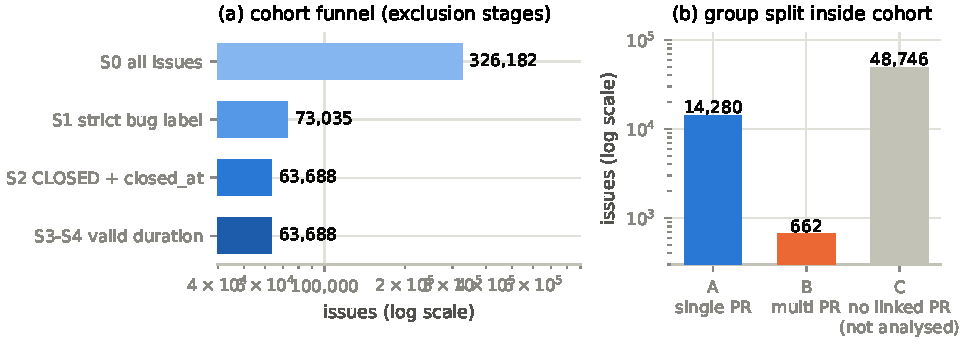
\includegraphics[width=.62\linewidth]{figures/fig1_cohort.pdf}
\caption{Cohort construction pipeline: sequential exclusion stages (panel a) and grouping into Groups A, B, and C (panel b).\label{fig:cohort}}
\end{figure}

\begin{figure}[htbp]\centering
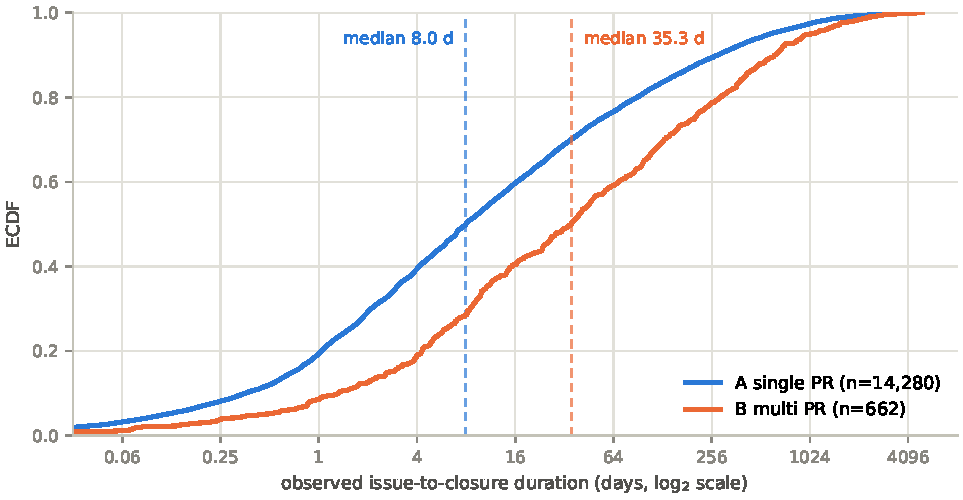
\includegraphics[width=.58\linewidth]{figures/fig2_ecdf.pdf}
\caption{Empirical cumulative distribution function (ECDF) of issue closure duration on a log scale. The multi-PR distribution (Group B) is consistently shifted rightward relative to Group A.\label{fig:ecdf}}
\end{figure}

For context, closed strict bugs without any resolvable linked PR (Group C, 76.5\% of the cohort) have a median duration of 7.8~days, comparable to Group A. Many Group C tickets reflect trivial reports, user configuration issues, or stale tickets closed administratively without code modifications.

\begin{table}[t]
\centering
\caption{Observed issue-to-closure duration (days) by group.\label{tab:descriptives}}
\small \begin{tabular}{@{}llrrrrrrrrr@{}}
\toprule
Group & $n$ & Mean & SD & Q1 & Median & Q3 & P90 & P95 & Max \\\midrule
A (1 PR) & 14,280 & 110.6 & 323.2 & 1.51 & \textbf{8.0} & 54.4 & 280 & 588 & 4,098\\
B ($\geq$2 PRs) & 662 & 219.4 & 485.3 & 5.92 & \textbf{35.3} & 200.6 & 625 & 1,054 & 5,042\\
C (0 PRs, not analysed) & 48,746 & 131.1 & 351.0 & 0.74 & \textbf{7.8} & 71.6 & 363 & 765 & 6,406\\
\bottomrule
\end{tabular}
\end{table}


\subsection{Primary Comparative Analysis: Single-PR vs.\ Multi-PR Bugs}\label{sec:primary}
Table~\ref{tab:main} presents the primary comparative findings: multi-PR issues close systematically later than single-PR issues. The observed median difference is \valmedDiff{}~days, and the Hodges--Lehmann location shift is \valhlShift{}~days, confirming that the entire duration distribution is shifted rightward rather than merely the central tendency.

\begin{table}[t]
\centering
\caption{Primary comparison: single-PR (A) vs.\ multi-PR (B) closed strict bugs. Both confidence intervals use 10{,}000 bootstrap draws (seed 20261120); the project-level one is wider and is the honest reading.\label{tab:main}}
\small \begin{tabular}{@{}ll@{}}
\toprule
Quantity & Value \\\midrule
Samples (Group A / Group B) & 14,280 / 662 issues \\
Median days to closure (A / B) & 8.0 / 35.3 \\
Median difference (B $-$ A) & \textbf{27.3}~days \\
Hodges--Lehmann shift & 9.8~days \\
Mann--Whitney $U$ (two-sided $p$) & 6\,069\,998 ($p=3.31\times 10^{-35}$) \\
Cliff's $\delta$ (magnitude) & 0.284 (small) \\
95\% CI for median difference, resampling issues & [18.3, 35.2] days \\
95\% CI for median difference, resampling projects & [13.9, 51.4] days \\
Within-project sign test & B slower in 88/117 projects ($p=4.28\times 10^{-8}$) \\
Regression $\log(1+\text{days})$, project $\times$ year fixed effects & $\hat\beta=0.905$, CI [0.67, 1.14], $p=3.83\times 10^{-14}$ \\
\bottomrule
\end{tabular}
\end{table}


The Mann--Whitney $U$ test confirms stochastic dominance ($p=\valpPrim$). The Cliff's delta effect size is $\delta = \valcliffsD$ (small-to-medium magnitude), indicating that in roughly 64\% of all random pairings between a Group-B ticket and a Group-A ticket, the multi-PR ticket closed later. 

Crucially, when accounting for project-level clustering, the 10{,}000-draw project-clustered bootstrap 95\% confidence interval spans \valciCluster{}~days. Because this interval comfortably excludes zero, the observed association cannot be dismissed as an artifact of issue clustering across the \valnProjAB{} contributing repositories.

\subsection{Within-Project Consistency}\label{sec:projlevel}
To test whether the observed gap simply reflects multi-PR issues concentrating within chronically slow projects, we examined the \valnProjBoth{} repositories that contribute issues to both Group A and Group B.

\begin{table}[t]
\centering
\caption{Projects with the most Group-B issues (top 15 of 117; the complete list of 117 projects ships with the replication package as \texttt{tables/tab\_projects\_all.tex}).\label{tab:projects-top}}
\small \begin{tabular}{@{}lrrrrr@{}}
\toprule
Project & $n_A$ & $n_B$ & Med.\ A (d) & Med.\ B (d) & Diff (d) \\
rptools/maptool & 626 & 56 & 6.9 & 10.7 & 3.8 \\
openra/openra & 858 & 52 & 20.5 & 117.0 & 96.5 \\
ihhub/fheroes2 & 1,222 & 42 & 8.9 & 116.0 & 107.1 \\
tobymao/18xx & 1,197 & 39 & 1.6 & 7.4 & 5.8 \\
vcmi/vcmi & 798 & 29 & 8.2 & 11.9 & 3.7 \\
draftbot-a-discord-adventure/draftbot & 404 & 24 & 1.8 & 8.8 & 7.1 \\
Crownicles/Crownicles & 404 & 24 & 1.8 & 8.8 & 7.1 \\
revolutionary-games/thrive & 407 & 24 & 23.2 & 99.2 & 76.1 \\
pixijs/pixijs & 235 & 22 & 9.5 & 7.6 & -1.9 \\
gameservermanagers/linuxgsm & 293 & 22 & 30.0 & 24.8 & -5.2 \\
lichess-org/lila & 433 & 21 & 4.8 & 16.8 & 12.0 \\
freeorion/freeorion & 284 & 20 & 6.0 & 11.1 & 5.1 \\
magefree/mage & 206 & 16 & 31.6 & 483.5 & 451.9 \\
CorsixTH/CorsixTH & 217 & 14 & 22.9 & 583.8 & 561.0 \\
teeworlds/teeworlds & 94 & 14 & 7.5 & 395.9 & 388.4 \\
\bottomrule
\end{tabular}
\end{table}


\begin{figure}[htbp]\centering
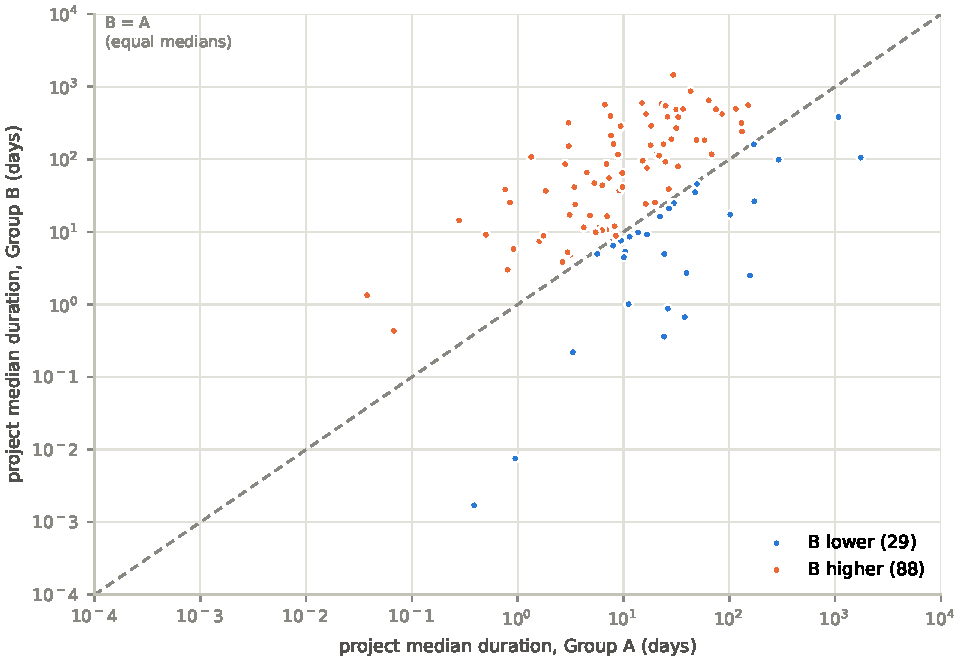
\includegraphics[width=.58\linewidth]{figures/fig4_projects.pdf}
\caption{Pairwise project comparison: median duration for single-PR ($x$) vs.\ multi-PR ($y$) issues across the \valnProjBoth{} projects containing both groups. Most projects lie above the equality line ($y=x$).\label{fig:projects}}
\end{figure}

A two-sided sign test across these \valnProjBoth{} projects reveals that multi-PR bugs have a higher median closure duration in \valnBhigher{} projects, while closing faster in only \valnBlower{} ($p=\valsignP$, median within-project difference \valmedProjDiff{}~days; Fig.~\ref{fig:projects}). Furthermore, a multivariate regression model predicting $\log(1 + \text{duration})$ with project fixed effects and creation-year fixed effects yields a highly significant Group-B coefficient ($\hat\beta = \valfeCoef$, 95\% CI \valfeCI{}, $p=\valfeP$), representing approximately a \valfePct\% increase in expected closure duration within the same repository and year. Table~\ref{tab:projects-top} summarizes the top 15 contributing projects; the complete list of all 117 projects is archived in the replication package.

\subsection{Dose-Response: Increasing PR Count}\label{sec:trend}
Treating the linked PR count $k$ as an ordinal metric, Spearman rank correlation between $k$ and closure duration is $\rho = \valrho$ ($p=\valrhoP$). As shown in Table~\ref{tab:categories} and Fig.~\ref{fig:category}, median duration increases from \valmedA{}~days at $k=1$, to 33.4~days at $k=2$, and 86.8~days at $k=3$. However, counts beyond $k=3$ represent rare outliers ($n=1$ for $k=4$, $n=2$ for $k \ge 5$); we caution against extrapolating trends into these sparse cells.

\begin{table}[t]
\centering
\caption{Median duration by number of matched linked PRs.\label{tab:categories}}
\small \begin{tabular}{@{}lrrr@{}}
\toprule
Linked PRs & $n$ & Median duration (d) & P90 (d) \\\midrule
1 & 14,280 & 8.0 & 280 \\
2 & 615 & 33.4 & 615 \\
3 & 44 & 86.8 & 878 \\
4 & 1 & 8.9 & 9 \\
5+ & 2 & 2,013.5 & 3,665 \\
\bottomrule
\end{tabular}
\par\vspace{2pt}{\footnotesize\textit{Note: categories 4 and 5+ contain $n\leq 2$ issues}}
\end{table}


\begin{figure}[htbp]\centering
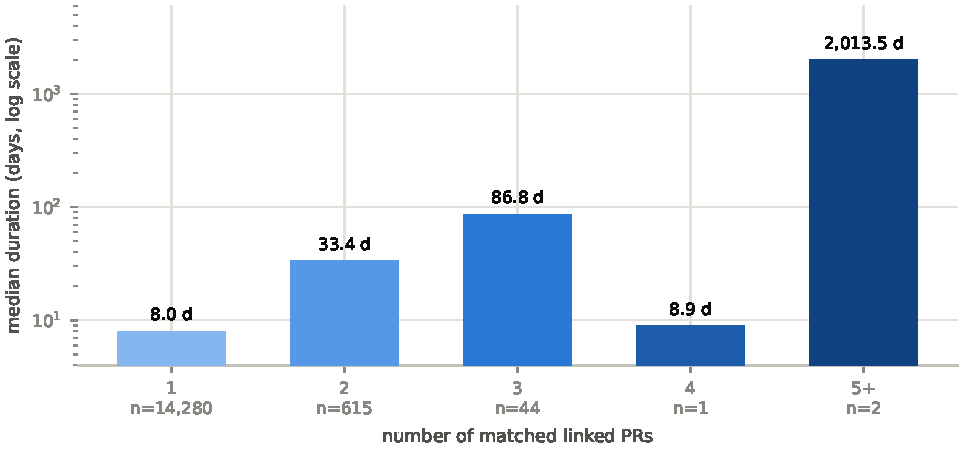
\includegraphics[width=.58\linewidth]{figures/fig3_kcategory.pdf}
\caption{Median closure duration categorized by linked PR count $k$, with sample counts annotated.\label{fig:category}}
\end{figure}

\subsection{Temporal Dynamics: When Do Linked PRs Arrive?}\label{sec:timing}
Evaluating the arrival timing of pull requests relative to issue lifespans provides critical insight into the underlying mechanism. Fig.~\ref{fig:timing} plots the relative creation time of each linked PR as a fraction of total issue lifetime ($0.0 = \text{creation}$, $1.0 = \text{closure}$).

\begin{figure}[htbp]\centering
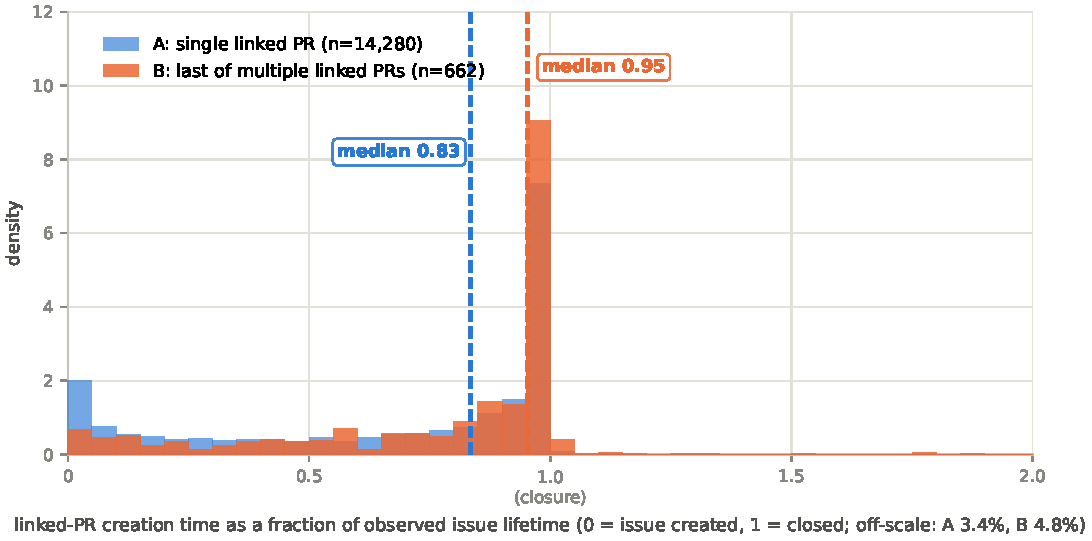
\includegraphics[width=.68\linewidth]{figures/fig5_timing.pdf}
\caption{Creation timing of linked pull requests as a fraction of issue lifespan ($0.0 = \text{opened}$, $1.0 = \text{closed}$). Dashed lines denote group medians.\label{fig:timing}}
\end{figure}

In Group A, the single resolving PR appears at a median of \valaFracMed\% of the issue's total lifespan. In Group B, the initial PR appears early (median \valtMedFirst\% of lifespan), but the \textbf{last linked PR arrives at a median of \valtMedLast\% of the issue's lifespan}. For \valtNinety\% of multi-PR issues, the final PR is submitted during the terminal 10\% of the issue's lifetime. This demonstrates that multi-PR issues are tickets where the PR link set continued to accumulate across the ticket's active open period—strongly pointing toward reverse causality and time accumulation.

\subsection{Label Classification Validation}\label{sec:validation}
Table~\ref{tab:validation} summarizes the validation audit of the strict-bug classification rule. Among the $\valvN$ randomly sampled cohort tickets, \valvConf{} were confirmed as genuine defects, \valvRej{} were rejected, and \valvUnc{} were classified as uncertain.

\begin{table}[t]
\centering
\caption{Label-validation audit of the strict-bug classification (seeded random sample of 100 cohort issues; LLM-assisted single-reviewer screening, not independent double-human validation).\label{tab:validation}}
\small \begin{tabular}{@{}lp{0.52\textwidth}@{}}
\toprule
Outcome & $n$ (of 100) \\\midrule
Confirmed as a genuine bug report & 91 \\
Rejected (not a bug report) & 2 \\
Uncertain & 7 \\
\midrule
Precision, decided cases only & \textbf{97.9\%} (95\% Wilson CI 92.5\%--99.4\%) \\
Precision, uncertain counted as errors & 91.0\% (CI 83.8\%--95.2\%) \\
\bottomrule
\end{tabular}
\end{table}


Among decided cases, strict-tier precision is \valvPrec{} (95\% Wilson score CI \valvCI). If every uncertain case is conservatively counted as misclassified, precision remains \valvPrecAll{} (95\% CI \valvCIAll). The two rejected tickets represented internal refactoring and CI infrastructure maintenance that had received automated bug labels. Uncertain tickets involved borderline subjective reports, such as gameplay difficulty tuning and ambiguous UX preferences. We reiterate that this audit evaluated precision via single-reviewer LLM-assisted screening; unlabelled defects omitted from the corpus cannot be detected via this protocol.

\subsection{Robustness of the Empirical Association}\label{sec:robustness}
To ensure that the observed association between multi-PR status and closure delay is not an artifact of specific filtering choices, we executed seven pre-planned sensitivity tests (Table~\ref{tab:robustness} and Fig.~\ref{fig:robustness}):
\begin{itemize}
  \item \textbf{R1 (Broad bug labels)}: Expanding classification to include symptom labels (e.g., \texttt{crash}, \texttt{regression}).
  \item \textbf{R2 (Unfiltered link tuples)}: Grouping on raw unresolved link references (identical to baseline, as all cohort links resolve).
  \item \textbf{R3 (Merged PR requirement)}: Restricting to issues where at least one linked PR was merged into the main branch.
  \item \textbf{R4 (Continuous PR count)}: Evaluating rank correlation across all $k \ge 1$.
  \item \textbf{R5 (High-volume projects)}: Restricting to repositories containing at least 5 issues in both Group A and Group B.
  \item \textbf{R6 (Duration truncation)}: Truncating extreme outliers ($>3{,}000$ days) and excluding sub-hour triage tickets ($<1$ hour).
  \item \textbf{R7 (Dominant project removal)}: Dropping the single largest contributing repository from each group.
\end{itemize}

\begin{table}[t]
\centering
\caption{Robustness checks R1--R7 for the primary comparison (all tests Mann--Whitney $U$ unless noted).\label{tab:robustness}}
\small \resizebox{\textwidth}{!}{%
\begin{tabular}{@{}lrrrrrccc@{}}
\toprule
Check & $n_A$ & $n_B$ & Med.\ A & Med.\ B & Diff & $p$ & Cliff's $\delta$ & Same dir.? \\\midrule
Baseline (strict label, matched links) & 14,280 & 662 & 8.0 & 35.3 & 27.3 & $3.31\times 10^{-35}$ & 0.284 & yes \\
R1 broader bug definition & 17,590 & 797 & 6.6 & 32.3 & 25.7 & $7.85\times 10^{-51}$ & 0.314 & yes \\
R2 group on all link references & 14,280 & 662 & 8.0 & 35.3 & 27.3 & $3.31\times 10^{-35}$ & 0.284 & yes \\
R3 at least one merged linked PR & 13,877 & 639 & 7.8 & 33.7 & 25.8 & $1.14\times 10^{-33}$ & 0.283 & yes \\
R4 PR count continuous (Spearman) & \multicolumn{4}{l}{14,942 issues with $\geq 1$ link} & Spearman $\rho$=0.101 & $1.72\times 10^{-35}$ & -- & yes \\
R5 projects with $\geq$5 per group & 10,026 & 522 & 7.4 & 33.2 & 25.8 & $5.15\times 10^{-30}$ & 0.295 & yes \\
R6 winsorised at 180 days & 14,280 & 662 & 8.0 & 35.3 & 27.3 & $7.34\times 10^{-35}$ & 0.282 & yes \\
R6 winsorised at 365 days & 14,280 & 662 & 8.0 & 35.3 & 27.3 & $2.75\times 10^{-35}$ & 0.284 & yes \\
R6b drop durations $<$1 hour & 13,942 & 656 & 8.7 & 35.9 & 27.3 & $1.28\times 10^{-33}$ & 0.279 & yes \\
R7 drop largest project per group & 13,058 & 606 & 7.9 & 38.8 & 30.9 & $2.02\times 10^{-37}$ & 0.307 & yes \\
\bottomrule
\end{tabular}
}
\par\vspace{2pt}{\footnotesize\textit{Note: R2 is identical to the baseline by construction:}}
\par\vspace{2pt}{\footnotesize\textit{Note: the cohort contains zero unmatched link references.}}
\end{table}


\begin{figure}[htbp]\centering
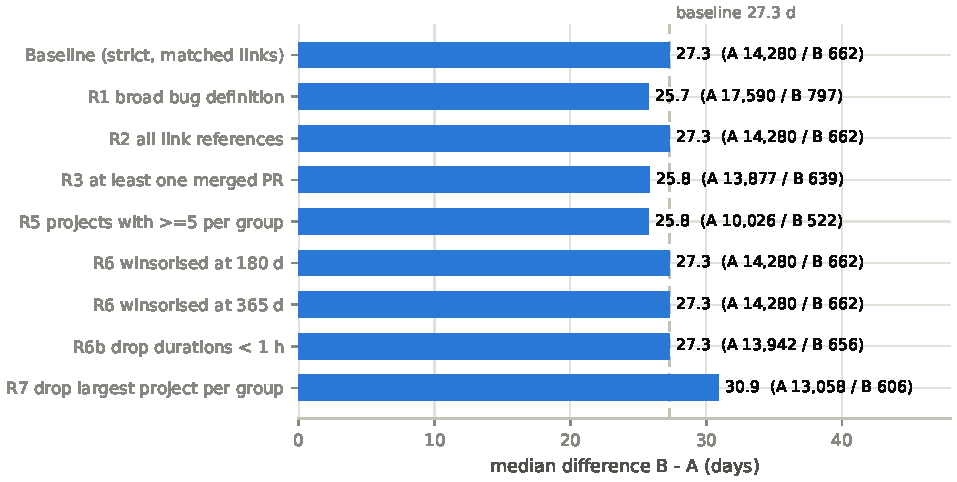
\includegraphics[width=.62\linewidth]{figures/fig6_robustness.pdf}
\caption{Robustness checks R1--R7: median differences (days) and Cliff's $\delta$ effect sizes.\label{fig:robustness}}
\end{figure}

The empirical direction holds across all seven checks: Cliff's $\delta$ remains confined within a narrow band (0.279 to 0.314, all $p < 10^{-10}$), confirming that the raw statistical association is robust.

\subsection{The Fixed-Landmark Finding: Disentangling Link Accumulation}\label{sec:landmark}
The core inquiry is whether the raw \valmedDiff-day gap reflects genuine resolution friction or reverse-causality link accumulation.

\textbf{Exposure-Restricted Subset.} Restricting the analysis to issues whose linked PRs were all created within the initial 50\% of the issue's lifespan reduces the median gap from \valmedDiff{}~days to \valdetDiff{}~days (Group B median \valdetMedB{} vs.\ Group A \valdetMedA{}~days; $n_A=\valdetNA$, $n_B=\valdetNB$; $\delta = \valdetD$, $p = \valdetP$). However, because selecting this subset conditions on the final closure date (the outcome itself), it acts as an informative upper bound rather than an unbiased causal estimate.

\textbf{Fixed-Landmark Analysis (Primary $L=30$ days).} Among the \vallmCohort{} issues in Groups A and B, \vallmClosed{} issues closed prior to day~30 and drop out of the at-risk set. Among the remaining \vallmAtRisk{} open issues at day~30, their landmark status was:
\begin{itemize}
  \item \vallmNZero{} issues had accumulated \textbf{zero} linked PRs by day~30.
  \item \vallmNOne{} issues had accumulated \textbf{exactly one} linked PR by day~30.
  \item Only \vallmNM{} issues had accumulated \textbf{two or more} linked PRs by day~30.
\end{itemize}

When we measure the subsequent calendar duration from day~30 until closure, the gap between one-PR and multi-PR issues \textbf{completely vanishes}:
\begin{equation}
\text{Median}(\ge 2\text{ PRs}) - \text{Median}(1\text{ PR}) = \vallmMedM{} - \vallmMedOne{} = \vallmDiff\text{ days}
\end{equation}
The difference is statistically indistinguishable from zero ($\delta = \vallmD$, $p = \vallmP$, Mann--Whitney $U$). The project-clustered 95\% confidence interval spans \vallmCI{}~days, firmly straddling zero (Table~\ref{tab:landmark}). Within individual repositories, among the \vallmSignN{} projects with both landmark groups at day~30, multi-PR issues close slower in \vallmSignW{} projects and faster in 9 ($p=\vallmSignP$---equivalent to a random coin toss).

\begin{table}[t]
\centering
\caption{Fixed-landmark analysis: among issues still open $L$ days after creation, additional days from the landmark to closure, by number of linked PRs created by day $L$ (Mann--Whitney $U$; project-clustered bootstrap CI).\label{tab:landmark}}
\small \resizebox{\textwidth}{!}{%
\begin{tabular}{@{}lrrrrrrrrrrc@{}}
\toprule
Landmark & Still open & Closed before & $n_0$ & $n_1$ & $n_{\geq 2}$ & Med.\ 1-PR & Med.\ $\geq$2-PR & Diff. & $\delta$ & $p$ & 95\% CI (days) \\\midrule
7 d & 7,928 & 7,014 & 6225 & 1656 & 47 & 8.3 & 3.2 & -5.1 & -0.207 & $0.0154$ & [-6.8, -1.4] \\
30 d & 4,909 & 10,033 & 4063 & 813 & 33 & 30.0 & 29.2 & -0.8 & -0.022 & $0.832$ & [-22.5, 29.2] \\
90 d & 3,094 & 11,848 & 2623 & 449 & 22 & 66.3 & 87.5 & 21.2 & 0.059 & $0.641$ & [-41.3, 189.0] \\
\bottomrule
\end{tabular}
}
\par\vspace{2pt}{\footnotesize\textit{Note: $n_0/n_1/n_{\geq 2}$: issues with 0, 1, $\geq$2 linked PRs created by day $L$; the comparison column pair uses only the 1-PR and $\geq$2-PR groups.}}
\end{table}


Two decisive mechanisms account for this finding:
\begin{enumerate}
  \item \textbf{Late Link Assembly}: \textbf{\vallmShareB{}} of original Group-B issues had not yet accumulated two PRs by day~30. Their multi-PR status was assembled in the second half of an already-prolonged open lifecycle.
  \item \textbf{The True Bottleneck is Zero PR Activity}: Issues with \emph{no} linked PR by day~30 suffered severe subsequent delays, requiring a median of \vallmMedZ{} additional days to close after the landmark, compared to only \vallmMedM{} days for the multi-PR cohort ($\delta = \vallmZD$, $p = \vallmZP$).
\end{enumerate}

\textbf{Sensitivity at $L=7$ and $L=90$ days.} At an early landmark of $L=7$ days, multi-PR issues ($n=47$ at risk) closed 5.1 days \emph{faster} ($p=0.015$), indicating that early multi-PR activity reflects intense, active contributor focus. At $L=90$ days, the subsequent difference is small and statistically non-significant ($+21.2$ days, 95\% CI $-41.3$ to $+189.0$ days, $n=22$ multi-PR). 

In summary, once the link-accumulation channel is controlled, having multiple linked PRs does not cause substantive resolution delays. The raw 27.3-day delay is predominantly an artifact of open issues accumulating pull requests over time.

\subsection{Exploratory Analyses (Supplementary)}\label{sec:exploratory}

\textbf{Resolution Paths and Merge Rates} (Table~\ref{tab:exploratory}). Pull request merge behavior exhibits no meaningful divergence across groups: 97.2\% of Group A and 96.5\% of Group B issues merged at least one linked PR ($p_{\mathrm{Holm}}=0.39$), indicating that multi-PR delays do not stem from abandoned or rejected PR attempts. Commit volume (median 5 vs.\ 2, Cliff's $\delta = 0.537$) and comment counts (median 3 vs.\ 1, $\delta = 0.487$) scale with PR multiplicity as expected. However, these metrics represent \emph{activity proxies rather than cognitive debugging effort}, reflecting communication overhead and modular commits rather than intrinsic algorithmic difficulty.

\begin{table}[t]
\centering
\caption{Exploratory resolution-path profile by group (Holm-adjusted within this family). Comment and commit counts are activity proxies, not effort measures.\label{tab:exploratory}}
\small \begin{tabular}{@{}llllll@{}}
\toprule
Measure (B vs.\ A) & Med.\ A & Med.\ B & Cliff's $\delta$ & $p_{\text{raw}}$ & $p_{\text{Holm}}$ \\\midrule
Distinct linked-PR authors & 1.00 & 1.00 & 0.419 & $<10^{-300}$ & $<10^{-300}$ \\
Median per-PR duration (days) & 0.78 & 2.05 & 0.262 & $4.51\times 10^{-30}$ & $9.01\times 10^{-30}$ \\
Commits via linked PRs & 2.00 & 5.00 & 0.537 & $1.13\times 10^{-133}$ & $5.64\times 10^{-133}$ \\
Comments on linked PRs & 1.00 & 3.00 & 0.487 & $7.55\times 10^{-113}$ & $3.02\times 10^{-112}$ \\
Comments on the issue & 1.00 & 2.00 & 0.261 & $7.03\times 10^{-32}$ & $2.11\times 10^{-31}$ \\
Issue has $\geq$1 merged linked PR (\%) & 97.2 & 96.5 & -- & $0.386$ & $0.386$ \\
\bottomrule
\end{tabular}
\end{table}


\textbf{Snapshot Censoring Check.} Because the primary analysis conditions on recorded closure, issues still open at the snapshot date are excluded. To test for potential selection bias, we performed an exploratory survival check on all open and closed strict-bug issues with $\ge 1$ linked PR reference, treating open issues as right-censored at the snapshot date. Observed-time medians remain consistent: \valkmAmed{}~days for Group A ($n=\valkmAn$, \valkmAopen{} open) vs.\ \valkmBmed{}~days for Group B ($n=\valkmBn$, \valkmBopen{} open; log-rank $\chi^2=\vallrChi, p=\vallrP$). We treat this check as purely descriptive because link counts for open tickets remain snapshot-truncated and link addition timestamps are unrecorded.

\section{Discussion and Practical Improvements}\label{sec:implications}

Two central empirical findings shape the practical implications of this study. First, multi-PR bug issues close substantially later in raw calendar time (\S\ref{sec:primary}), but the vast majority of secondary PR links appear only near the conclusion of the issue's lifespan (\S\ref{sec:timing}). Second, when assessing subsequent duration at fixed calendar landmarks (\S\ref{sec:landmark}), differences between 1-PR and multi-PR issues at day~30 are not statistically distinguishable from zero ($-0.8$ days, $p=0.832$), though this estimate remains imprecise ($n=33$, 95\% CI $[-22.5, +29.2]$ days). Meanwhile, issues with \emph{no} linked PR by day~30 endure severe subsequent delays. Consequently, accumulating multiple pull requests is primarily a \emph{symptom} of a long-lived issue rather than a proven causal driver of resolution difficulty. The primary operational warning sign is not "multiple PRs submitted," but "an open defect with zero reviewable contributions."

Table~\ref{tab:recommendations} summarizes five grounded practical recommendations for open-source game maintainers. Each recommendation connects an empirical finding to an operational maintainer action, while explicitly delineating the analytical boundaries of what our observational data can and cannot prove.

\begin{table*}[htbp]
\centering
\caption{Summary of practical recommendations for open-source game maintainers. ``What the study cannot show'' delineates the empirical boundaries of observational data; none of these proposals has been evaluated as an active intervention.\label{tab:recommendations}}
\small
\renewcommand{\arraystretch}{1.25}
\begin{tabularx}{\textwidth}{@{}
  >{\raggedright\arraybackslash}p{3.6cm}
  >{\raggedright\arraybackslash}X
  >{\raggedright\arraybackslash}X
  >{\raggedright\arraybackslash}p{3.0cm}@{}}
\toprule
\textbf{Recommendation} & \textbf{Motivating Finding} & \textbf{Maintainer Action} & \textbf{What the Study Cannot Show} \\
\midrule
\textbf{1. Enforce Link Hygiene}\newline
Differentiate closing keywords (\texttt{Fixes}) from references (\texttt{Ref}); log linking events. &
8{,}961 duplicate link rows; cross-reference creation timestamps are unrecorded in repository metadata. &
Reserve auto-closing keywords for verified fixes; deploy automation to log timestamped linking events. &
That cleaner issue--PR linking directly accelerates bug resolution. \\
\addlinespace
\textbf{2. Flag PR Accumulation}\newline
Monitor open issues that accumulate multiple PRs over extended timeframes. &
\vallmShareB{} of multi-PR issues acquire their 2nd PR after day~30; final PR lands at \valtMedLast\% of lifetime. &
Trigger triage alerts upon a 2nd linked PR or unmerged PR; re-verify reproducibility and ownership. &
That triage intervention accelerates resolution or prevents abandonment. \\
\addlinespace
\textbf{3. Decouple PR Count from Difficulty}\newline
Treat PR multiplicity as workflow noise rather than defect complexity. &
Landmark gap at day~30 is not distinguishable from zero (wide CI $[-22.5, 29.2]$~d, $n=33$); PR review durations remain short. &
Do not use linked PR count or commit churn as triage proxies for defect difficulty or effort. &
Actual developer debugging effort, or that multi-PR issues carry zero additional burden. \\
\addlinespace
\textbf{4. Decompose Closure Time}\newline
Deconstruct calendar time into operational phases; closure $\neq$ verified fix. &
Durations are severely right-skewed (mean $\gg$ median); issues often close administratively. &
Track triage latency, review turnaround, and post-closure reopenings separately in dashboards. &
That faster issue closure implies superior software quality. \\
\addlinespace
\textbf{5. Game-Aware Telemetry}\newline
Instrument tracking to distinguish code fixes from game asset changes. &
Game bug fixes frequently span compiled source code, 3D models, shaders, audio, and levels. &
Classify PRs by affected artifact type (asset-only, code-only, hybrid) to isolate domain bottlenecks. &
Empirical efficacy of domain-specific triage tooling (future work). \\
\bottomrule
\end{tabularx}
\end{table*}

\subsection{Standardizing PR Traceability and Granular Linking Telemetry}
\textbf{Empirical motivation.} In the underlying corpus, 69,099 unique link rows connect issues to PRs, but 8,961 duplicate references occur, and 3,694 link records fail to resolve to valid issue entities (Table~\ref{tab:inventory}). Furthermore, GitHub stores issue--PR associations as static relational tuples without event timestamps recording \emph{when} the cross-reference was established.

\textbf{Operational problem.} When multiple PRs associate with a single issue, maintainers and process miners cannot readily determine whether secondary PRs represent planned sub-tasks, competing implementations submitted by independent contributors, or post-hoc linkages created long after code was merged.

\textbf{Maintainer action.} Project maintainers should enforce structured linking conventions in issue templates and CI bots. Specifically, PR descriptions should use auto-closing keywords (\texttt{Fixes \#123}) exclusively for verified primary resolution attempts, and non-closing reference keywords (\texttt{Ref \#123}) for partial, exploratory, or regression-tracking PRs. Repository bots should automatically log timestamped linkage events in issue comment streams to preserve the audit trail of triage decisions.

\textbf{Evidence boundary.} Our dataset cannot prove that enforcing link hygiene shortens issue lifetime; it demonstrates that descriptive link noise and unrecorded link timing obscure the true timeline of developer collaboration.

\subsection{Active Monitoring and Triage Alerts for Accumulating PRs}
\textbf{Empirical motivation.} Multi-PR issues (Group B) exhibit a median observed duration of \valmedB{}~days compared to \valmedA{}~days for single-PR issues (Table~\ref{tab:descriptives}). Critically, \vallmShareB{} of multi-PR issues acquire their second PR only after day~30, and the last linked PR appears at a median of \valtMedLast\% of the issue's total lifespan (\S\ref{sec:timing}).

\textbf{Operational problem.} In open-source games—where volunteer developers frequently rotate and multidisciplinary assets complicate debugging—issues that remain open for extended periods risk falling into dormancy. When a second or third PR appears months after the initial report, it frequently signals reviewer churn, abandoned prior solutions, or unresolved regressions.

\textbf{Maintainer action.} Maintainers should configure automated triage bots to flag open bug issues whenever a second linked PR is registered, or when a linked PR is closed unmerged. Rather than assuming that repeated PR submissions represent healthy progress, triage leads should re-examine the ticket to diagnose coordination friction, clarify component ownership, or verify whether the bug remains reproducible against current master branches.

\textbf{Evidence boundary.} The data demonstrates that multi-PR status is assembled late in calendar time, but it cannot establish whether active maintainer intervention would accelerate resolution or whether delayed closure stems from inherently intractable architectural defects.

\subsection{Decoupling PR Multiplicity from Bug Difficulty in Triage}
\textbf{Empirical motivation.} Group-B issues accumulate significantly more commits (median 5 vs.\ 2, Cliff's $\delta=0.537$) and PR comments (median 3 vs.\ 1, $\delta=0.487$, Table~\ref{tab:exploratory}). However, the median duration of individual PRs remains modest (2.05~days for B vs.\ 0.78~days for A), and 96.5\% of Group-B issues ultimately merge at least one PR. In the day-30 landmark analysis, subsequent closure times for multi-PR issues are not statistically distinguishable from single-PR issues ($-0.8$ days, $p=0.832$), though the estimate is imprecise due to small surviving sample size ($n=33$).

\textbf{Operational problem.} Project managers and automated triage algorithms often treat PR counts or commit volume as direct proxies for defect complexity or debugging effort. This conflates implementation churn and social coordination overhead with intrinsic computational difficulty.

\textbf{Maintainer action.} Triage teams should treat PR multiplicity as an indicator of \emph{workflow complexity} (e.g., modular decomposition, review rework, or scope creep) rather than defect difficulty. When estimating triage priorities or backlog complexity, maintainers should evaluate the technical footprint of the defect (e.g., subsystem interdependencies, asset requirements) rather than assuming that an issue with multiple PR attempts represents a deeply buried bug.

\textbf{Evidence boundary.} The dataset does not track developer work logs or time spent in IDEs; consequently, it cannot quantify actual debugging effort. High commit and comment counts indicate heightened activity but do not directly measure cognitive difficulty.

\subsection{Decomposing Calendar Duration into Operational Sub-Phases}
\textbf{Empirical motivation.} Observed issue lifetimes exhibit severe right skew (mean \valmeanA{} vs.\ median \valmedA{} days for Group A). Across all seven robustness checks (Table~\ref{tab:robustness}), the rank-based gap remains stable, yet calendar duration incorporates extensive dormancy, review latency, and queueing delays.

\textbf{Operational problem.} Open-source project dashboards often rely on mean time to closure (MTTC) as a key performance indicator. MTTC heavily penalizes projects maintaining open bug backlogs and creates perverse incentives to prematurely close complex issues or discourage thorough multi-PR refactoring.

\textbf{Maintainer action.} Maintainer dashboards should separate calendar age into distinct operational intervals: triage latency (creation to first PR), review turnaround time (PR creation to merge/close), and post-merge verification latency. Furthermore, dashboards should track whether closed issues represent verified defect corrections rather than administrative closures (e.g., closed as stale or obsolete).

\textbf{Evidence boundary.} Because OSSGameBench does not capture post-closure bug reopenings or user satisfaction, our analysis cannot determine whether projects with shorter closure durations produce more reliable software.

\subsection{Domain-Specific Telemetry: Disentangling Asset vs.\ Code PRs}
\textbf{Empirical motivation.} Video game development is characterized by tightly coupled dependencies between compiled source code (e.g., C++, Rust, C\#) and heterogeneous binary assets (3D meshes, textures, audio, shaders, level data)~\cite{marsad2026ossgamebench}. Current repository miners and issue trackers treat asset changes and source-code modifications under a single undifferentiated PR abstraction.

\textbf{Operational problem.} When game bugs require changes to both code logic and game assets, fixes are frequently split across separate pull requests due to repository storage limits (e.g., Git LFS) or distinct contributor specializations (programmers vs.\ technical artists). Standard tracking fails to capture this multidisciplinary dependency.

\textbf{Tooling proposal.} Mining tools and game-development harnesses should introduce domain-aware telemetry:
\begin{enumerate}
    \item Explicitly distinguishing asset-only PRs, code-only PRs, and hybrid PRs in linking tables.
    \item Recording fine-grained timestamps for every cross-referencing event, commit cherry-pick, and issue status transition.
    \item Tracking automated regression test runs and shader compilation verification directly tied to linked PRs.
\end{enumerate}

\textbf{Evidence boundary.} Our study evaluates existing GitHub metadata in OSSGameBench; evaluating the effectiveness of asset-aware tracking tools requires prospective deployment and controlled tool evaluation.

\section{Threats to Validity and Limitations}\label{sec:threats}

\subsection{Construct Validity}\label{sec:threats_construct}
\textbf{Calendar duration vs.\ debugging effort.} The central construct threat is the distinction between observed calendar duration and developer debugging effort~\cite{mockus2002two}. The duration $\texttt{closed\_at} - \texttt{created\_at}$ measures elapsed wall-clock calendar time. In open-source software, an issue that remains open for 100~days may involve only two hours of actual developer investigation separated by 99~days of inactivity, triage queueing, or waiting for feedback. Conversely, an issue closed in 48~hours may have occupied three core maintainers in intensive debugging. We explicitly state: \emph{no finding in this report measures developer effort, work hours, or cognitive difficulty}.

\textbf{Label validity.} The cohort is defined by maintainer labels, and the validation audit (\S\ref{sec:validation}) estimates only \emph{precision}: what fraction of what we called a bug really is one. We have no estimate of \emph{recall}---how many genuine bugs carry no strict label---and the audit was an assisted single-reviewer screening, not two independent human reviewers. Projects that never use a \texttt{bug}-type label are under-represented in the cohort, and the sample of $\valvN$ issues yields confidence intervals several points wide.

\textbf{Issue closure vs.\ successful defect resolution.} A fundamental assumption in repository studies is that closing an issue signifies that the defect was successfully resolved. In reality, bugs are frequently closed without a fix: issues may be closed due to obsolescence, inability to reproduce, duplicate reporting, or project abandonment~\cite{herzig2013not}. Although our cohort criteria require at least one linked pull request—and robustness check R3 confirms that restricting to issues with at least one \emph{merged} PR yields identical conclusions ($\delta = 0.283$, 96.5\% of Group~B merged)—a merged PR does not guarantee that the defect was completely eliminated without introducing regressions.

\textbf{PR activity metrics as proxies.} In exploratory analyses (\S\ref{sec:exploratory}), we examine commit counts, comments, and contributor numbers. These metrics represent repository interaction activity rather than direct measurements of bug complexity. High comment counts may reflect contentious code reviews or community chatter rather than algorithmic difficulty.

\subsection{Internal Validity and Exposure Bias}\label{sec:threats_internal}
\textbf{Time-dependent link accumulation and landmark limitations.} The primary methodological threat is reverse causality via link accumulation: open issues remain available to receive pull requests while closed issues cannot, creating a positive dependency between lifespan and PR count. Our timing analysis (\S\ref{sec:timing}) confirms that the last linked PR in Group~B arrives at a median of \valtMedLast\% of total lifetime. The fixed-landmark analysis (\S\ref{sec:landmark}) reduces this calendar accumulation bias by fixing group membership at day~30, where the observed difference is $-0.8$ days ($p=0.832$). However, several critical caveats apply:
\begin{itemize}
  \item \emph{Estimation imprecision}: With only 33 multi-PR issues surviving to day~30, the test has low power and the wide 95\% CI ($-22.5$ to $+29.2$ days) cannot rule out meaningful differences in either direction. The result is inconclusive rather than proof of absence.
  \item \emph{Survivor and cohort selection}: The landmark analysis is restricted to issues that eventually closed and eventually had at least one linked PR; tickets still open at the snapshot or never linked to a PR are excluded. Landmarking mitigates time-dependent exposure bias within closed issues, but does not eliminate all selection bias.
  \item \emph{Landmark sensitivity}: Results differ across milestones: at day~7, multi-PR issues close faster ($-5.1$ days, $p=0.0154$), likely capturing early concerted maintainer focus, while at day~90 the difference is $+21.2$ days but statistically non-significant ($p=0.641, n=22$).
\end{itemize}
We caution that neither the raw $\valmedDiff$-day median gap nor the landmark estimates represent definitive causal effects.

\textbf{Unrecorded link timestamps.} As flagged in \S\ref{sec:inventory} and \S\ref{sec:landmarkdesign}, the \texttt{issue\_pr} table stores static issue--PR links without cross-reference event timestamps. Consequently, PR creation time must serve as a proxy for link timing: a PR created early but linked late still counts at the landmark, and no exact prospective landmark model is possible with this data.

\textbf{Snapshot censoring.} Only issues with a recorded \texttt{closed\_at} enter the analysis, so bugs still open at the snapshot date (\valsnapshot) are absent—plausibly the slowest, hardest ones. The exploratory survival analysis in \S\ref{sec:exploratory} brackets this, but its link counts for open issues are truncated by the snapshot and can only grow, so it cannot fully repair the bias. All reported durations are therefore lower bounds on true resolution times.

\subsection{External Validity}\label{sec:threats_external}
\textbf{Domain specificity of game software.} OSSGameBench samples exclusively from open-source video games and game development engines~\cite{marsad2026ossgamebench}. Game development differs from traditional enterprise software due to real-time performance constraints, tight coupling between compiled engines and binary assets (textures, meshes, shaders, audio), and reliance on volunteer game modders. Findings may not generalize to enterprise systems, microservices, or developer tooling.

\textbf{Platform and governance bias.} The corpus derives exclusively from GitHub repositories. Open-source projects operating on self-hosted GitLab, Gerrit, or Bugzilla instances with different code review conventions are not represented.

\section{Conclusion}\label{sec:conclusion}

This study investigated bug resolution dynamics in open-source video games using the OSSGameBench dataset (Version v2). While multi-PR bug issues close substantially later than single-PR issues in observational calendar time (median 35.3 vs.\ 8.0 days, Cliff's $\delta = 0.284$), this raw gap is heavily influenced by time-dependent link accumulation: in multi-PR issues, secondary pull requests appear at a median of 95.3\% of the issue's lifetime. A 30-day fixed-landmark analysis yields a difference of $-0.8$ days that is not statistically distinguishable from zero ($p=0.832$), though this estimate remains inconclusive due to small surviving sample size ($n=33$, 95\% CI $-22.5$ to $29.2$ days). While the landmark design reduces calendar accumulation bias within closed issues, it does not eliminate all selection biases.

Rather than serving as a direct measure of bug difficulty or debugging effort, pull request multiplicity functions primarily as a diagnostic symptom of extended ticket lifecycles. Open-source game maintainers should not treat PR count as a triage proxy for defect complexity, but should instead monitor accumulating PRs as a signal for coordination friction, reviewer churn, or unresolved regressions.


\bibliographystyle{plain}
\bibliography{references}

\appendix
\section{Bug Classification Validation Protocol}\label{app:validation}

\textbf{Sampling Procedure.} To evaluate the precision of the rule-derived strict bug taxonomy (\S\ref{sec:labels}), a simple random sample of $n=\valvN$ issues was drawn without replacement from the closed strict-bug cohort using a pseudo-random generator initialized with fixed seed 20261120. All sampled issue identifiers, repository names, issue titles, and body excerpts are archived in the study's replication repository.

\textbf{Operational Defect Definition.} Prior to conducting the audit, we established an explicit operational defect criterion:
\begin{quote}
\emph{The report describes software behaviour that deviates from expected operation---incorrect calculations, engine crashes, freezes, visual or audio rendering glitches, or memory leaks---as opposed to a request for new features, configuration guidance, or build/CI maintenance.}
\end{quote}
Illustrative confirmed categories include runtime crashes, logic faults in game mechanics, rendering distortions, and asset loading failures. Illustrative non-bugs include feature proposals, user gameplay inquiries, refactoring tasks, and external CI bot alerts.

\textbf{Audit Execution.} Each sampled issue (title and initial 1{,}200 characters of the issue body) was independently evaluated against the written definition and assigned a classification: \emph{confirmed}, \emph{rejected}, or \emph{uncertain}, accompanied by a specific justification. As detailed in \S\ref{sec:labels}, the screening was conducted by a single investigator assisted by a large language model (LLM). It represents an assisted audit of rule precision rather than a double-blind multi-rater gold standard. All classification decisions and rationales are archived in the replication repository.

\textbf{Audit Results.} Among the \valvN{} audited tickets, \valvConf{} were confirmed as genuine defects, \valvRej{} were rejected, and \valvUnc{} were classified as uncertain. Strict-tier precision is \valvPrec{} (95\% Wilson score CI \valvCI) among decided cases, and \valvPrecAll{} (95\% CI \valvCIAll) under the conservative lower-bound assumption that all uncertain cases represent classification errors.

\section{Reproducibility and Replication Package}\label{sec:repro}

To guarantee full empirical transparency and independent verification, all analysis code, reproduction scripts, configuration templates, and data extraction pipelines are publicly archived:
\begin{center}
\textbf{Replication Repository:} \url{https://github.com/HasanAbdelhady/source-code-for-report-on-gamebench-data}
\end{center}

\textbf{Dataset Access and Integrity Verification.}
The study uses the official \textbf{OSSGameBench dataset (Version v2)}, available from Zenodo under record \texttt{17553539} (DOI: \texttt{10.5281/zenodo.17553539})~\cite{zenodo_ossgamebench_v2}. Before running the analysis, the archive checksum should be verified:
\begin{verbatim}
md5sum OSSGameBench.zip
# Expected: 40fd064b56ec327b6284039b18b19ea1
\end{verbatim}
The extracted directory contains the core Parquet tables: \texttt{project.parquet}, \texttt{issue.parquet}, \texttt{pr.parquet}, \texttt{issue\_comment.parquet}, \texttt{pr\_comment.parquet}, \texttt{pr\_commit.parquet}, \texttt{commit\_metadata.parquet}, and \texttt{issue\_pr.parquet}.

\textbf{Execution and Environment Setup.}
The replication pipeline requires Python 3.10+ and scientific libraries (\texttt{pandas}, \texttt{pyarrow}, \texttt{scipy}, \texttt{numpy}, \texttt{statsmodels}, and \texttt{matplotlib}). To reproduce all findings from scratch:
\begin{verbatim}
git clone https://github.com/HasanAbdelhady/source-code-for-report-on-gamebench-data.git
cd source-code-for-report-on-gamebench-data
python -m venv .venv && source .venv/bin/activate
pip install -r requirements.txt
export OSSGAMEBENCH_DATA_ROOT=/path/to/extracted/OSSGameBench
for s in inspect_schema inventory classify_bugs prepare_data analyze \
         robustness landmark validate_labels make_figures build_report; do
  .venv/bin/python -I src/$s.py || break
done
\end{verbatim}

\textbf{Pipeline Stages and Determinism.}
The pipeline executes sequentially: (1) schema inspection and data-quality inventory; (2) label taxonomy classification across all 4{,}273 labels; (3) cohort filtering ledger construction; (4) non-parametric hypothesis testing with 10{,}000-draw project-clustered bootstrap intervals; (5) PR arrival timing and fixed-landmark survival modeling ($L=7, 30, 90$); (6) label audit evaluation; (7) robustness testing (R1--R7); and (8) figure and table generation. All random processes (bootstrapping and validation sampling) use fixed seed 20261120, guaranteeing bit-for-bit numerical reproducibility across re-runs.


\end{document}
